%\begin{frame}{Opgave 4: Grafisk undersøgelse}
%    Lav en grafisk undersøgelse af fejlen $\lvert f(x)-p_N(x) \rvert$, for en række forskellige værdier af N baseret på en modificeret udgave af \textsc{Interpolation bin.py.}
%\end{frame}

\begin{frame}{Grafisk undersøgelse}
    Det ses, at approximationen passer til funktionen ved nogle værdier for $N$, herunder $N = 45$. 
    Ved andre indsatte værdier opstår store udsving i yderpunkterne i definitionsmængden $[0,3]$.
    Dette stemmer overens med forlæsningsnoterne fra kursusgang $5(s.4-5)$, hvor der kan ses, at Runge har bevist, at yderpunkterne divergerer.
    %
    \begin{figure}[h!]
    \begin{center}
    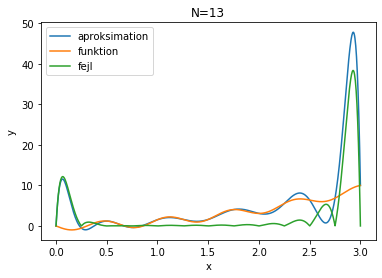
\includegraphics[scale=0.5]{images/N=13.png}
    \end{center}
    \caption{$N = 13$ - Eksempel på Runges Fænomen.}
    %
    \end{figure} 
\end{frame}

\begin{frame}{Grafisk undersøgelse}
    \begin{figure}[h!]
    \begin{center}
    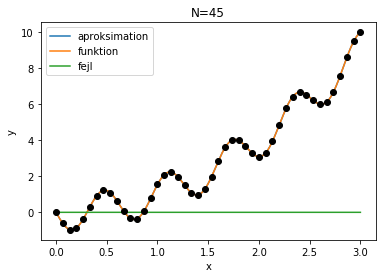
\includegraphics[scale=0.5]{images/N=45.png}
    \end{center}
    \caption{$N = 45$ - Eksempel på overensstemmelse.}
    %
    \end{figure}
\end{frame}

\begin{frame}{Grafisk undersøgelse}
    \begin{figure}[h!]
    \begin{center}
    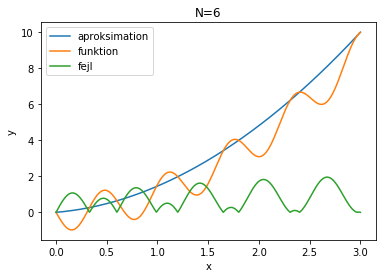
\includegraphics[scale=0.5]{images/N=6.png}
    \end{center}
    \caption{$N = 6$ - Eksempel på at approximationen ikke stemmer overens med funktionen, og at fejlen dermed bliver høj.}
    %
    \end{figure} 
    
\end{frame}